\section{Math\-Function Class Reference}
\label{classMathFunction}\index{MathFunction@{MathFunction}}
{\tt \#include $<$utils.h$>$}

Inheritance diagram for Math\-Function::\begin{figure}[H]
\begin{center}
\leavevmode
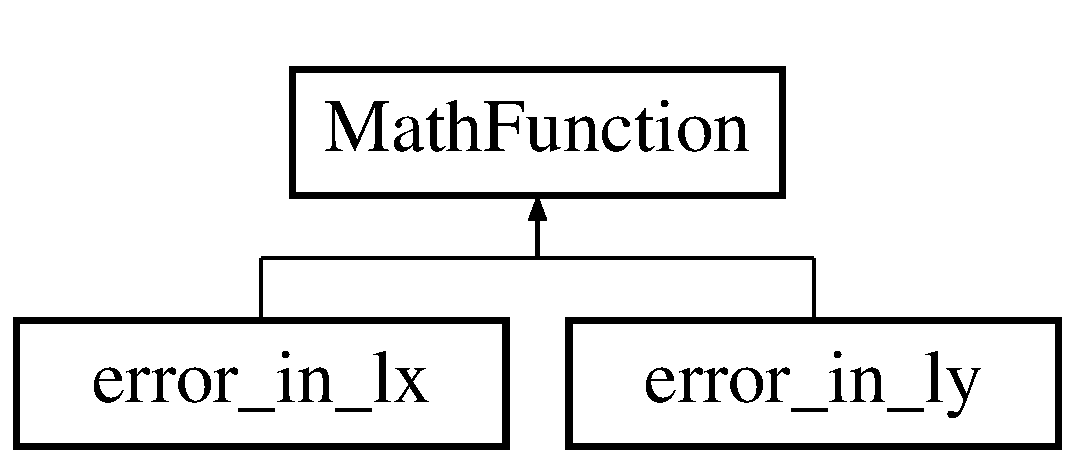
\includegraphics[height=2cm]{classMathFunction}
\end{center}
\end{figure}
\subsection*{Public Member Functions}
\begin{CompactItemize}
\item 
virtual double \textbf{call} (double x)=0\label{classMathFunction_5c0978bd3e24e8647784eed17f11e25d}

\end{CompactItemize}


\subsection{Detailed Description}
Template class for a generic function of the form: f:R-$>$R

An instance of a subclass of this must be used as the argument to minimise\_\-function 



Definition at line 77 of file utils.h.

The documentation for this class was generated from the following file:\begin{CompactItemize}
\item 
utils.h\end{CompactItemize}
